\chapter{Introduction}
\label{ch:intro}

It has been long understood that living organisms are complex, composed of highly connected and interdependent systems working in concert to give rise to unique biological features and carry out discrete biological functions. However, system-wide studies tended to remain largely theoretical until recent decades. Now, state-of-the-art technologies are able to generate data in quantities that were once inconceivable by traditional approaches and which have finally made system-level investigations possible. With this vast volume of biological data, component parts (e.g., nucleic acids, proteins, and lipids) can be pieced together to elucidate how biological entities interact to carry out coordinated functions and how a system might fail and cause disease. 

Many computational approaches have been developed for the study of biological data and among them, network-based approaches have become major ones. For instance, proteins are essential to nearly all cellular and molecular processes and only rarely do they act in isolation. By sequences of molecular events, such as the phosphorylation of a protein by another protein kinase, protein interactions form the scaffold for cellular responses, such as ensuring cell growth at a normal pace, unlike the abnormal rate in cancer \parencite{silverbush2019}. By modelling these interactions, such as in protein protein interaction networks, we can improve our understanding of protein functions and cellular responses, elucidate disease etiology arising from aberrant functioning, and discover targets for disease. 

This chapter introduces several concepts related to the types, measurements, modelling, storage and analyses of biological data. In particular, models which represent biological data within the context of their interactions and associations are given special focus, as are pathway and network-level analyses of various types of \textit{-omics} data in the biomedical domain. The publications which follow in later chapters detail the challenges in understanding complex biological systems, outline techniques for the interpretation of biological data and present methods for their investigation.

\section{Biological data representations}
\label{intro_1}

\subsection{Biological data}

Advanced technologies have accelerated the rate at which biological data is produced. Next generation sequencing (NGS), microarrays, and mass spectrometry (MS) are among the major technologies used to characterize and quantify the complete (or partially complete) profiles of distinct classes of biological entities. With these developments, different stages in the transfer of genetic information, from DNA to RNA to protein, can now be holistically and rapidly measured along with other biological data modalities, such as metabolites \parencite{hsiao2009}. The study of these profiles for a particular investigated molecular space is referred to as an \textit{omics} study, providing a global survey of the state of a certain type of entity at any given point in time. 

\textit{Omics} studies are especially valuable as investigating the complete profiles of biological entities can help to elucidate normal cellular functioning and processes that lead to observable phenotypes. Furthermore, perturbations to a system can be evident in different ways at the molecular level. Investigating the alterations that are caused by such perturbations can help to decipher the etiology of disease. One can, for example, characterize the complete expression profile of a sample in various contexts and/or conditions and ask how expression varies from one context to another, whether there are differences between conditions, or how a perturbation, such as by a drug, can affect a system at large. Currently, several branches in this field investigate various biological data types, the most common of which are introduced below \parencite{hasin2017, manzoni2018, lightbody2019, cai2022}.

\begin{figure}[ht]
    \centering
	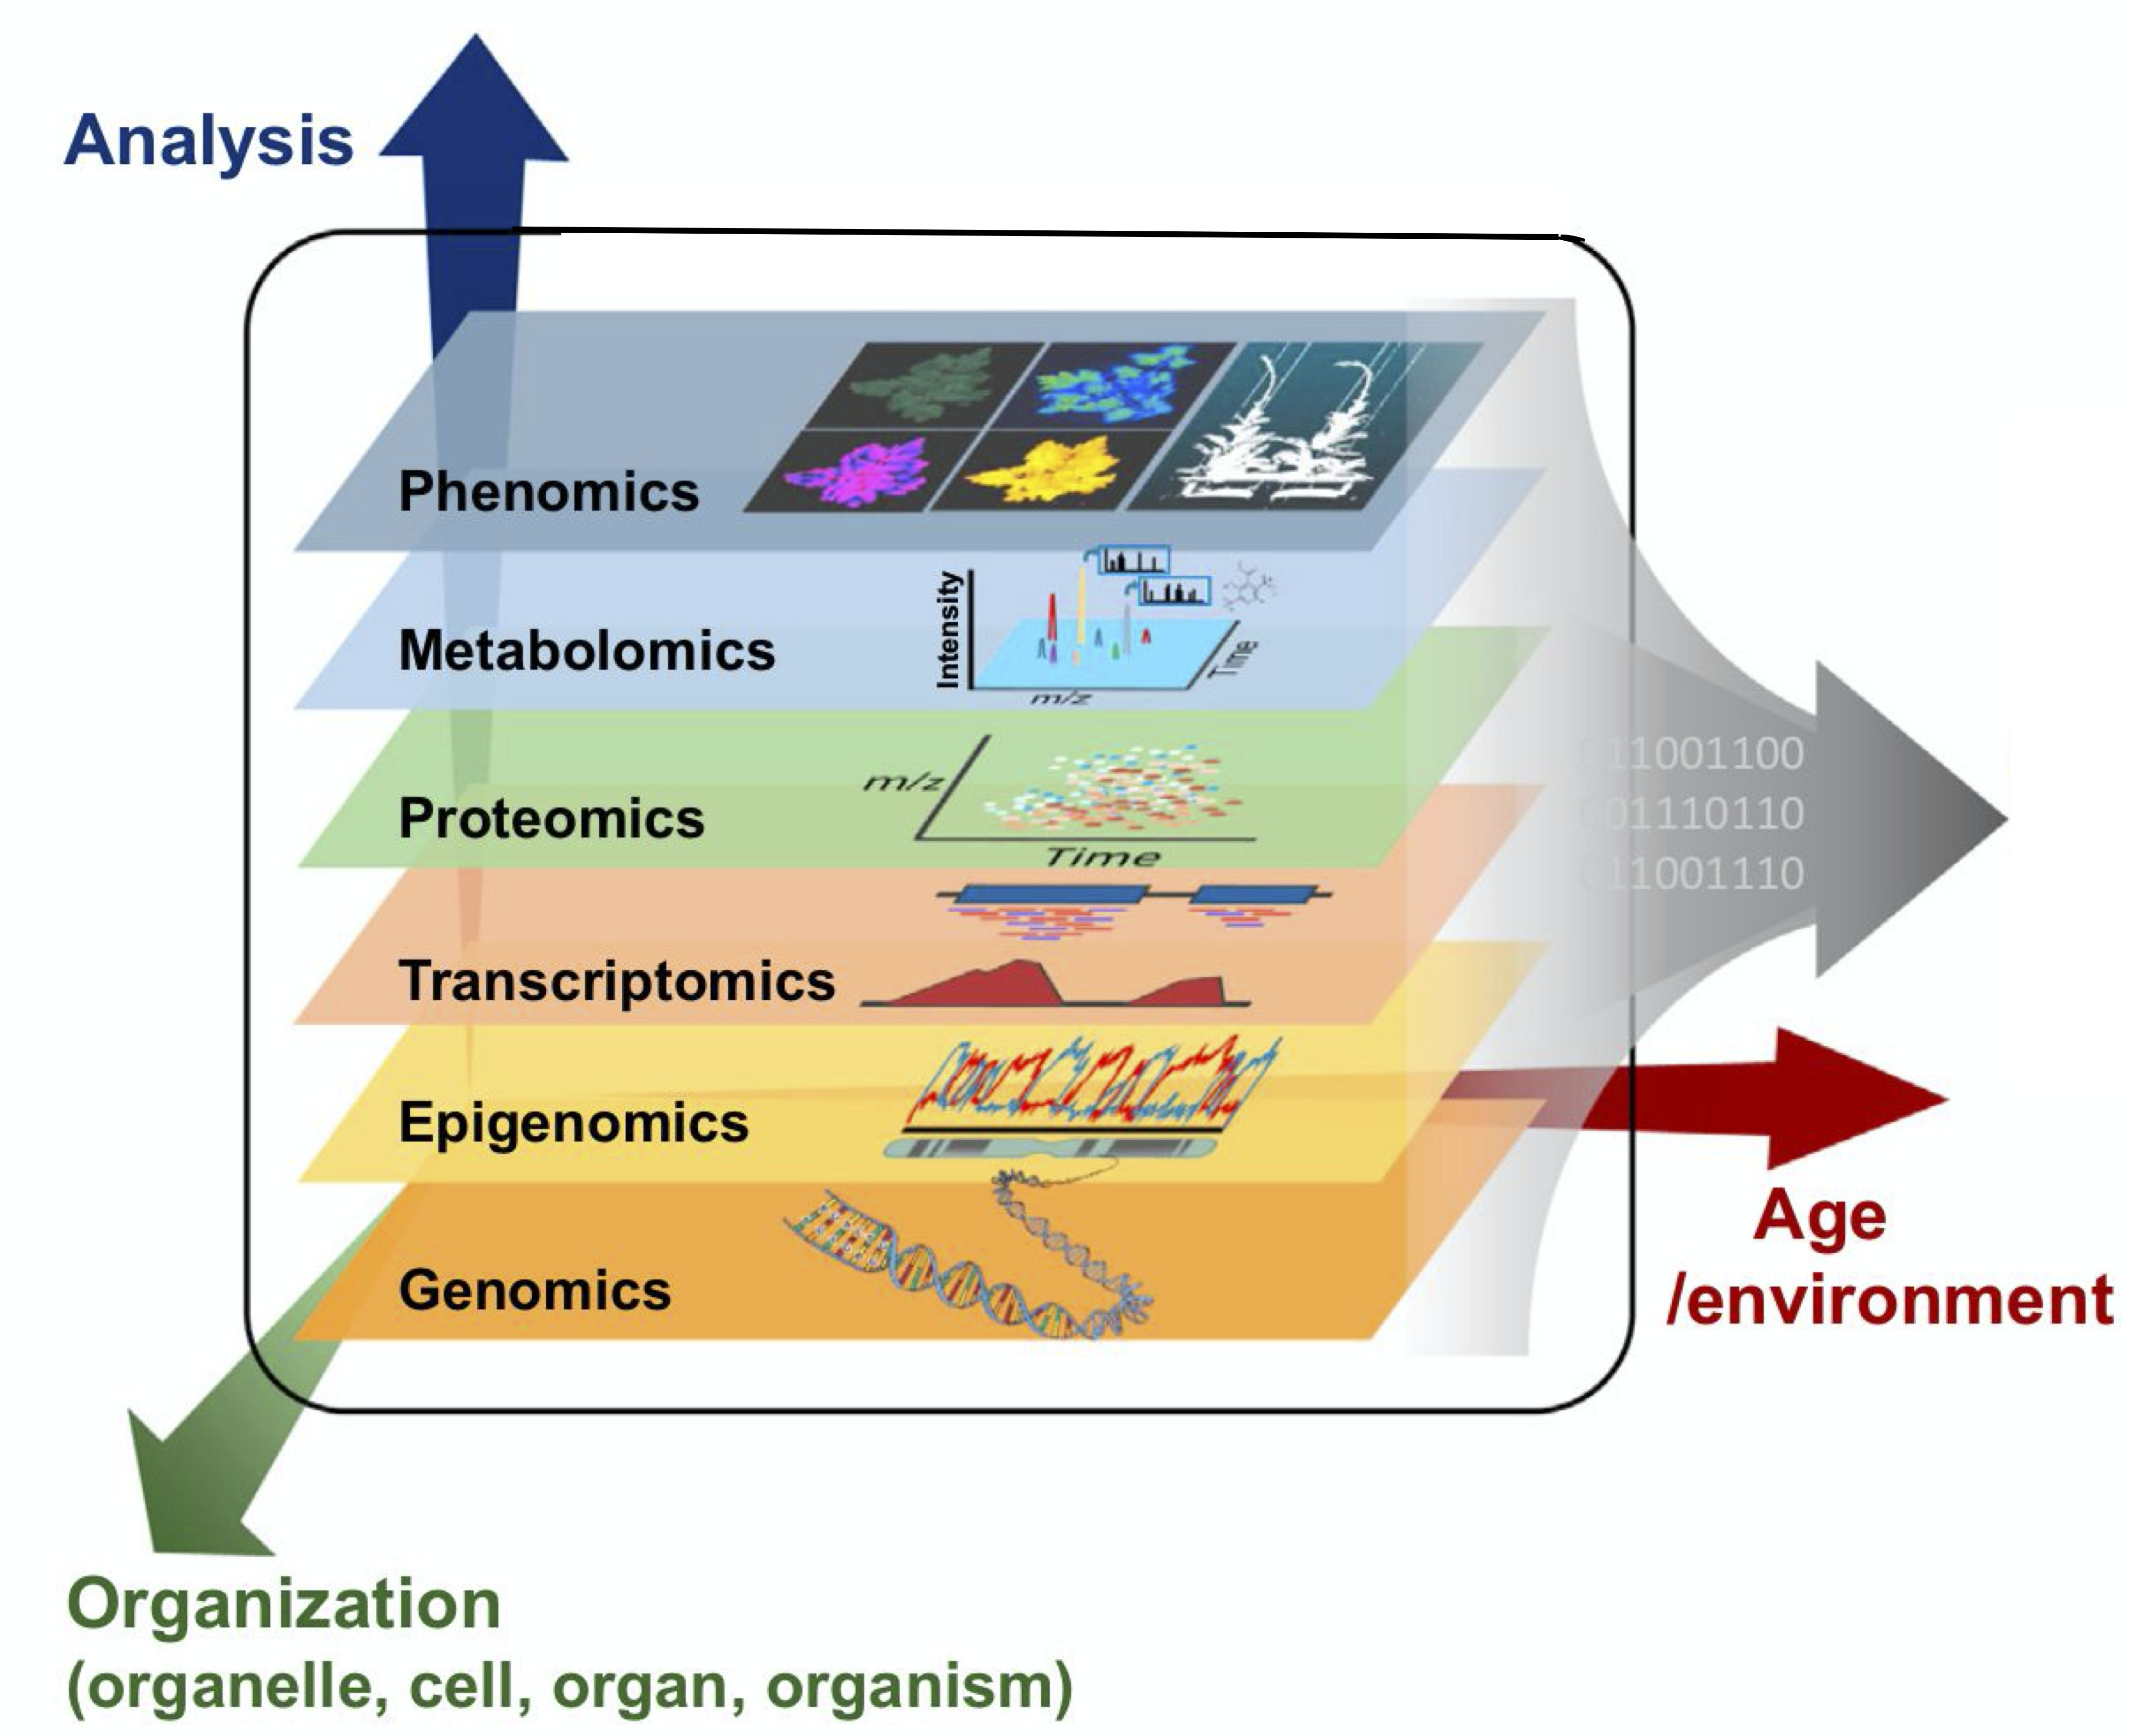
\includegraphics[width=\linewidth]{figures/omics_levels.png}
	\caption{\footnotesize \textbf{\textit{Omics} disciplines.} \textit{Omics} studies at increasingly complex levels of  biological organization. Image source: taken from \parencite{kim2016}.}
\end{figure}

\begin{itemize}
    \item   \textbf{Genomics.} The field of genomics was the first of many \textit{omics} disciplines to emerge. Focusing on the study of the complete genetic information of an organism (i.e., its genome), genomic experiments are used to identify associations between genetic variants and diseases as well as other phenotypes. The genome itself includes coding regions, genes which make up 1-2\% of the entire genome, and non-coding regions, constituting the remaining 98-99\% of DNA. Technologies associated with genomic data include DNA microarrays as well as NGS, such as whole genome sequencing (WGS), whole exome sequencing (WES), chromatin immunoprecipitation followed by sequencing (ChIP-seq) and single cell DNA sequencing (DNA-Seq). With these technologies, variations in the genome, such as single nucleotide variants (SNVs), insertions and deletions (indels), inversions, and copy number variations (CNVs) are routinely characterized. These data can be denoted by binary values, indicating that a gene is either wild type or mutated. While the vast majority of variants are benign, others may influence susceptibility to a disease or cause disease altogether, signifying the critical importance of their examination.
    
    \item   \textbf{Epigenomics.} While genomics focuses on sequence data, epigenomics is the study of the epigenome, specifically, all chemical modifications to the genome that do not change the nucleotide sequence itself. This particular \textit{omics} field is intended to investigate epigenetic modifications that play a key role in gene regulation (e.g., DNA methylation and histone modifications) as well as other processes. Notably, altered DNA methylation profiles have been noted in many diseases and can be used as disease biomarkers, for example in cancers, neuro-developmental disorders, metabolic disorders and autoimmune diseases \parencite{heyn2012}. Technologies for epigenomics include NGS (e.g., ChIP-seq) and array-based ones. 
    
    \item   \textbf{Transcriptomics.} Transcriptomics is concerned with the steady-state level of all mRNA transcripts of each gene. In this case, RNA sequences (or signals) are quantified and the abundance of RNA transcripts, or gene expression levels, are measured using technologies such as microarrys, RNAseq and single cell RNA-Seq (scRNAseq). The complete set of transcripts in a cell are collectively known as the transcriptome, including coding and non-coding RNAs, with coding RNA (mRNA) comprising 1-4\% of the transcriptome. It is important to note that although RNA transcript or gene expression levels are often used as proxies to infer protein expression levels and gene activity, they may not accurately reflect either of these \parencite{grant2007}. Although bulk RNAseq has been the predominant technology used to measure average global gene expression, bulk transcriptomic data can mask heterogeneity in cellular composition and cell types may also be sampled in varying proportions \parencite{li2021}. To offset these potential confounds and more accurately characterize the functional repertoire of individual cells, technological advancements within the past decade have resulted in the exponential scaling of scRNAseq experiments, now allowing for the parallel profiling of hundreds of thousands of individual cells in a single study \parencite{svensson2018} that can be stored in cell atlases, such as the Human Cell Atlas \parencite{karlsson2021}. 
    
    \item   \textbf{Proteomics.} Proteomics focuses on the study of the proteome, the complete set of proteins expressed in an organism, cell or tissue at a given point in time. Technologies, such as array-based and MS (although, primarily the latter) quantify protein abundance. The functions of many proteins are regulated by post-translational modifications (ex. phosphorylation, methylation, acetylation). These modifications affect various biological processes, such as the regulation of gene expression, signal transduction and DNA repair, and play key roles in various protein functions, including regulating enzyme activity and cell structure maintenance \parencite{ramazi2021}. Due to these modifications and additional factors, protein abundances can differ from the abundance of RNA transcripts, leading to some inaccuracies in inferring protein expression levels from gene expression levels. Compared to genomics and transcriptomics, proteomics tends to be a far more complex investigation owing to the large number of possible combinations of amino acids, polypeptide conformations and post-translational modifications of the resulting, functional protein. Finally, a single gene can encode for many proteins (e.g., due to alternative splicing), leading to a discrepancy between the total number of proteins (which tend to be much greater) than the total number of genes. 
    
    \item   \textbf{Metabolomics.} Metabolomics is concerned with the study of the metabolome, all metabolites which are the small molecule substrates and products of cellular processes in a biological system (e.g., carbohydrates, lipids, amino acids). Metabolites play a key role in cell functioning, including signal transduction and energy production. These molecules (e.g., ATP, acetyl-CoA) can regulate post-translational modifications (such as those described above) which affect protein activity, while the interaction of some metabolites with proteins can enable cellular responses through the initiation of signalling cascades \parencite{johnson2016}. When metabolite concentrations are outside of the normal range, these can be indicative of aberrant states. Analytical techniques associated with metabolomics include nuclear magnetic resonance (NMR) and MS-based technologies, which can be used to quantify all measurable metabolites, including unknown ones \parencite{roberts2012}. 
    
    \item   \textbf{Other biological data types.} Another rapidly expanding field is microbiomics, the study of microorganism communities (such as those of bacteria, viruses, fungi and their genes) of a particular system. The human microbiota alone is estimated to contain 38 trillion bacteria, alluding to the complexity of the microbiome \parencite{sender2016}. The impact of these microbes on human health are increasingly being discovered, with roles in cancer, disease susceptibility, infant health, anxiety, mood, cognition, and pain, amongst other indications \parencite{mohajeri2018, ursell2012}. Common techniques associated with microbiomics include 16S ribosomal (rRNA) sequencing and shotgun metagenomics sequencing to extract DNA from microbial samples. Besides discrete biological entities, fields such as radiomics also exist for the examination of  other biological data types, such as medical images from radiological modalities (e.g., computed tomography (CT), magnetic resonance (MRI), positron emission tomography (PET)), that can be converted into high-dimensional data for quantitative feature extraction \parencite{gillies2016}.
\end{itemize}

While \textit{omics} studies have provided insights that have already been put into clinical practice, (e.g., the identification of disease biomarkers \parencite{kim2010, baylin2001} and the characterization of disease progression \parencite{govender2021}), the disparate study of \textit{omics} data modalities can fail to comprehensively capture the complexity of biological systems, which essentially can occur as interactions of discrete biological entities across multiple \textit{omics} layers \parencite{yugi2016}. This has led to the emergence of multi-\textit{omics} experiments, where multiple \textit{omics} technologies are combined to generate integrated \textit{omics} data \parencite{karczewski2018,misra2019,hasin2017}. Several resources and platforms which integrate diverse \textit{omics} data types have become available, such as ColPortal for methylation, transcriptomic, microbiomic and clinical data, among other types, for colon cancer patients \parencite{esteban2019, conesa2019}.

\subsection{Molecular interactions} \label{interactions}

Individual biological entities, such as those described in the preceding section, rarely act in isolation to carry out biological functions. Instead, interactions, referring to the physical or functional association of two biological entities which cause or result in some biological effect, are the main drivers of cellular and molecular functions. These interactions can occur between the same types of entities (e.g., protein-protein interactions), across modalities (e.g., protein-metabolite interactions) as well as across biological constructs (e.g., gene-phenotype interactions) and can be divided into various classes, some of which are described below \parencite{gomez2020,sonawane2019,hawe2019}.

\begin{itemize}
    \item   \textbf{Protein-protein interactions} (PPIs) are stable or transient physical interactions between proteins which can result in the formation of a protein complex or a specific, temporary response, respectively. PPIs can be experimentally obtained via methods such as yeast-2-hybrid assays, MS-based approaches, or co-immunoprecipitation, while computational approaches for obtaining PPIs include prediction methods (e.g., homology-based interaction inference) or literature text-mining. PPI interaction resources include STRING \parencite{szklarczyk2021}, BioGrid \parencite{oughtred2019} and APID \parencite{alonso2019}. 

    \item   \textbf{Regulatory interactions} refer to the binding of proteins (i.e., transcription factors (TFs)) to certain regions of DNA which enhance or repress the expression of one or more genes and cause a change in their activity. Various experimental methods can be used to characterize TF-DNA binding, such as ChIP-seq, while databases which house these interactions include ReMap \parencite{hammal2022} and TRUUST \parencite{han2018}. 

    \item   \textbf{Metabolic reactions} are biochemical interactions that occur between metabolites and enzymes. These reactions result in the conversion of metabolites from one form to another, with each step in the conversion process mediated by specific enzymes, which catalyze these reactions. Databases of metabolic reactions include KEGG \parencite{kanehisa2000}, MetaCyc \parencite{caspi2014}, ENZYME \parencite{bairoch2000} and BRENDA \parencite{chang2021}. 
    
    \item   \textbf{Other types of interactions.} Other types of molecular interactions include signalling reactions, where post-translational modifications of one protein by another initiate a biological signal or transmit a signalling cascade, and interactions between metabolites and proteins, such as a drug and its protein target, where the metabolite can cause some alteration to the activity of the protein. However, these protein-metabolite interactions can be difficult to characterize due to their transient nature and weak affinities. MS- and NMR- based approaches have nonetheless been used to systematically map protein-metabolite interactions \parencite{li2020,diether2019}.
\end{itemize}

Various disease states can occur in the event of disruptions to normal interaction behaviours. For example, certain mutations in transcription factors (e.g., gene amplification, gene deletions and point mutations) can modify the regulatory circuits of a cell and are known to contribute to several diseases (e.g., cancers, autoimmune disorders, cardiovascular diseases and diabetes) \parencite{lee2013,lambert2018,bushweller2019}. An example lies with the oncogenic transcription factor, TAL1, whose binding with GATA3 and RUNX1 form a positive autoregulatory loop, driving an altered circuitry that likely contributes to the oncogenic human T cell acute lymphoblastic leukemia program \parencite{sanda2012}. 

\subsection{Interactomes}

Sets of molecular interactions can be arranged into what is known as an interactome, a network of molecular interactions between biological entities. Generally, the interactome is most often used to refer to sets of PPIs, such as the human interactome for all PPIs in humans cells. Nonetheless, interactomes of entities from other \textit{omics} layers have also been established, such as the human protein-DNA interactome (i.e., gene regulatory network) \parencite{hu2009}, RNA interactome \parencite{lin2020},  protein-RNA network \parencite{lapointe2015}, as well as the gene-interaction network of indirect, functional relationships between genes. By generating these interactomes, it becomes possible to model complete networks of interactions between individual biological entities to facilitate an understanding of their collective roles in normal and aberrant cellular functions.

\subsection{Context-specificity of interactions}

While the elucidation of molecular interactions and their representation within interactome networks is a significant step in modelling the complexity and interplay of entities within a functional, biological system, an important caveat is that interactions, and by extension, interactomes, tend to be void of biological context. For instance, in a study by Stacey \textit{et al.} \parencite{stacey2018}, the authors found no evidence for the occurrence of anywhere between 19 to 55\% of interactions reported in several literature-curated PPI databases. Thus, a molecular interaction may only be a snapshot of an event occurring in a particular cell and/or condition at a given point in time.

Although the cells of an organism contain the same DNA sequence, different cells can exhibit distinct behaviours and characteristics (e.g., a neuron vs. a white blood cell). These differences result from the specific binding of TFs to particular positions on the DNA sequence, resulting in variable levels of expression of particular genes and the diversity observed across different cell types. Consequently, this can mean that the conditions in which an experimental molecular interaction occurred may not be reflective of the actual interaction occurring within a given context (e.g., cell type or tissue). 

\section{Biological pathways}

While the interactomes described in the preceding section comprised sets of all interacting biological entities, a more knowledge-based approach to representing biological data is by collating sets of interactions into biological pathways. These pathways are essentially series of interactions between physical biological entities (or biological constructs) which result in a particular event, such as a cellular change or the formation of a product \parencite{pathways2020}. Collectively, pathways carry out some biological process \textbf{(see Figure \ref{pathways})}. For example, a biological pathway can represent how a signal is transmitted from an external to an internal environment, a particular carbohydrate is metabolized, DNA is repaired, or how a pathogen affects a host cell. Types of pathways which can be modelled include metabolic, signal transduction, gene regulation and disease pathways.

Not surprisingly, representing biological data in this simplified abstraction does imply some loss of information, such as spatio-temporal features. Furthermore, pathway representations can include interactions characterized in disease states \textit{in vitro} (e.g., HeLa cancer cell line), which although may be appropriate for the study of disease pathways, may not be generalizable to normal states. For example, interactions characterized in immortalized or tumorigenic fibroblasts in cell signalling pathways can be inherently biased and ill-suited to represent normal cellular functioning. Despite these shortcomings, pathways are advantaged by their capacity to formalize and abstract well-established relationships with literature validation, and by their ability to facilitate a visual and more easily interpretable understanding of complex processes. They are additionally advantaged by their capability to represent biological entities and constructs across multiple scales (e.g., from genotype to phenotype), and encode rich relationship descriptions (e.g., activation, inhibition, binding/association, phosphorylation) \parencite{joshi2005}.

{\footnotesize
\begin{figure}[ht]
	\centering
		\includegraphics[width=\linewidth]{figures/metro_map.png}
	\caption{\footnotesize \textbf{Biological pathway map.} Image source: taken from \parencite{chakazul2020}.}
    \label{pathways}
\end{figure}
}

Deconstructing the mechanisms by which a particular biological function is executed, not at the level of individual entities, but rather, considering their interplay as a whole, can serve several advantages. This includes understanding how individual entities assemble into modules to carry out discrete functions, as well as disease etiology. For example, this component mapping can help to identify pathways that are dysregulated by a disease as well as affected routes along specific pathways in order to reveal potential therapeutic targets.

\subsection{Pathway databases}

Given the popularity of pathway maps for the representation of biological data, a particular class of databases have emerged to formalize, collect and store biological pathways. Several academic and commercial enterprises have produced pathway databases numbering in the hundreds, reflecting the diversity of biological processes occurring in living organisms \parencite{bader2006}.

Many of these databases can be distinguished by the domains that they cover,  with some pertaining to a particular species (e.g., EcoCyc \parencite{keseler2017}, Plant Reactome \parencite{naithani2020}), or disease (e.g., NeuroMMSig \parencite{domingo2017}, AlzPathway \parencite{mizuno2012}, Atlas of Cancer Signalling Network (ACSN) \parencite{kuperstein2015}), while others differ by their content, such as those focused on signalling (e.g., SIGNOR \parencite{perfetto2016}, NetPath \parencite{kandasamy2010}) or metabolic pathways (e.g., MetaCyc \parencite{caspi2014}, BRENDA \parencite{chang2021}). Additionally, some databases can be highly specific (e.g., YTRP \parencite{yang2014} for transcriptional regulatory pathways in \textit{Saccharomyces cerevisiae}), while others are more comprehensive, covering hundreds or thousands of pathways across multiple species, such as KEGG \parencite{kanehisa2000}, Reactome \parencite{jassal2020}, WikiPathways \parencite{martens2021}, and PathBank \parencite{wishart2020}.

Besides differences in their content, pathway databases can also be distinguished by several other factors. For example, pathways across databases can be described in varying levels of detail such that some biological entities and/or interactions may be included within a pathway in a particular database, but excluded in the same pathway in another database \parencite{domingo2018, domingo2019}. Additionally, the average number of pathways in a given database can range from several hundred (e.g., KEGG), to over a hundred thousand (e.g., PathBank), hinting at variable definitions of pathway boundaries. The interconnected nature of biological pathways (as alluded to in \textbf{Figure \ref{pathways}}) also implies arbitrary definitions of pathway boundaries, which can be variously selected by domain experts for disparate databases. For instance, one database may define a particular biological process as a single pathway, while another database may define several parts of that same biological process as individual functional modules and separate pathways. One possible solution to standardize pathway definitions lies with a technique proposed by Belinky \textit{et al.,} \parencite{belinky2015} that uses hierarchical clustering and nearest neighbour graph representation to group similar pathways. Although the approach they use has been intended for merging pathways, it can also be used as an objective standard to define pathway boundaries, where boundaries are drawn to minimize redundancy across associated gene sets. In summary, even well-established, canonical pathways can differ across databases due to the aforementioned sources of variability, implying a degree of subjectivity in abstracting pathway knowledge. 

\subsection{Standard formats for interaction data }

Pathways are essentially computational data models which describe interactions between heterogeneous biological entities and/or constructs. In order to transform interaction data into pathways, several languages have been made available and are variously used by disparate pathway databases. Below, we provide a brief overview of various formats which have been adopted by the scientific community.

Among the most commonly used interaction formats are BioPAX and SBML. Biological  Exchange, or BioPAX, is a standard RDF/OWL- based language that can be used for the representation of various molecular and genetic interactions, pathways, and gene regulatory networks \parencite{demir2010}. BioPAX is established as a major pathway exchange format for the integration, visualization and analysis of pathway data. Databases which offer BioPAX export include Reactome, MetaCyc and WikiPathways. The Systems Biology Markup Language (SBML) is a standard XML-based language that is used to represent computational models of system biology \parencite{hucka2003}. Much like BioPAX, SBML is also intended as an exchange format and to describe various biological processes, such as metabolic and signalling pathways, with a particular focus on representing biochemical network models. Reactome, BRENDA, MetaCyc and PANTHER are among the databases which provide SBML export. 

Apart from the languages mentioned thus far, additional interaction formats that have been widely used include BEL, SBGN, PSI-MI, RDF and SIF. Similar to the above mentioned languages, Biological Expression Language (BEL) formalizes biological relationships in a computable form, and also includes rich, contextual-descriptions of causal and correlative relationships across biological scales \parencite{slater2012}. Systems Biology Graphical Notation (SBGN) has also been developed as an unambiguous standard for the representation, storage, visualization and exchange of biological processes \parencite{novere2009}, while the Proteomics Standards Initiative Molecular Interactions (PSI-MI) \parencite{hermjakob2004} exchange format is especially popular among databases of protein-protein interactions, such as IntAct \parencite{del2022}, BioGRID \parencite{oughtred2021} and MINT \parencite{calderone2020}. Finally, the triple structure (i.e., subject, predicate and object) of the Resource Description Framework (RDF) is also used as a standard model to represent biological relationships \parencite{miller2018}, while the Simple Interaction Format (SIF) can be used to generate networks from lists of molecular interactions. 

\subsection{Enabling interoperability across formats}

Although collectively, pathway databases cover a broad scope of information in varying levels of detail, due to a diversity of formats and the lack of interoperability between them, they tend to be fairly disconnected and only independently accessible to researchers. In addition, standardized nomenclature for pathways are lacking, further hindering pathway interoperability. Although some efforts have been made to standardize pathway nomenclature, as with the Pathway Ontology for the annotation of genes to pathway terms for multiple species \parencite{petri2014}, these have not yet been widely adopted. Despite these challenges, several software converters have been developed for the translation of one language to another (e.g., PathMe  \textbf{(Figure \ref{overlay})} \parencite{domingo2019}, PAX2GRAPHML \parencite{moreews2021}, PaxTools \parencite{demir2013}). Furthermore, meta-data databases, such as PathwayCommons \parencite{rodchenkov2020} and ConsensusPathDb \parencite{herwig2016}, have also been established to consolidate pathway knowledge and interaction data across several primary resources and represent data in a standardized format. These integrative approaches can serve to provide a far more holistic view of the knowledge surrounding a particular process and more accurately represent literature findings as opposed to the knowledge any singular resource may accumulate. 

{\footnotesize
\begin{figure}[ht]
	\centering
		\includegraphics[width=\linewidth]{figures/pathway_overlay.png}
	\caption{\footnotesize \textbf{Pathway overlay.}  Illustrations of the mTOR signaling pathway in multiple pathway databases (i.e., KEGG, Reactome  and WikiPathways) depicted in the three lowest layers, and their merged representation depicted in the topmost layer.}
    \label{overlay}
\end{figure}
}

\subsection{Pathway analysis}

A prototypical method for the interpretation of high dimensional biological data has become pathway enrichment analysis, a term which encapsulates a group of analytical methods that investigate whether a pathway is enriched, or over-represented, within a list of genes \parencite{reimand2019}. Typically, these genes are derived from a high throughput experimental dataset associated with a given phenotype. These analyses are primarily intended to garner mechanistic insights on large volumes of biological data by using pathway representations that can summarize high dimensional information (e.g., thousands of genes) to a handful of biological processes. A question that is commonly addressed by a pathway analysis is whether specific sets of genes may be associated with a given phenotype or biological process. 

Despite advances in available pathway enrichment methods, the vast majority discard topological pathway information. Instead, a pathway is simplified to a set of genes without any interaction information (i.e., a gene set), and the gene set is tested against differentially expressed genes from an experimental dataset that investigates a particular phenotype (e.g., breast cancer versus normal) \parencite{maleki2020}. More specifically, a common pipeline for several enrichment methods is to first obtain a ranking of genes according to their degree of differential expression. Each gene set within a collection or from a pathway database is then tested to determine whether genes in the gene set are over-represented at the top and/or bottom of the ranked list of genes. If the genes of the gene set are clustered at either the top and/or bottom of the ranked list more so than expected by chance, the gene set may be statistically significant for the particular phenotype under study. If, however, the genes within the gene set are equally distributed throughout the ranked list, this suggests that the gene set is unlikely to be interesting or relevant in some statistically significant way to the investigated phenotype \parencite{subramanian2005,hung2012}. The results procured from such an analysis can thus shed light on biological processes that may be affected by a particular condition which may otherwise go unnoticed if an experimental dataset were to be examined solely at the gene level rather than the pathway level. 

\section{Network biology}

The networks described thus far (e.g., the interactome and biological pathways) all fall within the framework of network biology, the abstraction and mathematical depiction of relationships between biological entities and/or concepts \parencite{liu2020}. The field concerned with the modelling of pairwise relationships between objects such as these is formally referred to as graph theory. In the sections that follow, we introduce key definitions and concepts within graph theory, as well as network-based methods and their applications in computational network biology. 

\subsection{Graph theory and definitions}

A graph can be defined as \textit{G} = \textit{(V, E)}, where \textit{V} is a set of vertices that represent nodes and \textit{E} is a set of edges that represent connections between nodes. Standard data structures to represent graphs are through collections of adjacency lists or through adjacency matrices. Adjacency list-based representations are particularly suited for sparse graphs, though an adjacency matrix representation may be preferred in cases when a graph is dense, or for efficient lookup of edge connections between specific vertices. There exist several classes of graphs which are typically defined by their edge types, as described in Table \ref{graphs}  \parencite{pavlopoulos2011,mason2007,cormen2022}.

Of the types of molecular interactions described in subsection \ref{interactions}, PPIs are typically modelled in undirected graphs, representing symmetric binding relationships, while metabolic reactions, signalling reactions, and regulatory interactions are frequently modelled as causal edges in directed graphs. Edges in an undirected weighted graph can be used to model the strength of correlated expression of genes in one type of biological network, termed co-expression networks \parencite{langfelder2008}. Applications of bipartite graphs can include the representation of enzyme-reaction links, gene-disease links and drug-target links \parencite{pavlopoulos2018}. Finally, biological applications of hypergraphs can include the modelling of metabolic reactions, where many substrates are converted into many products.

\begin{table}[ht]
\raggedleft
\begin{tabularx}{\textwidth}{lX}
\hline
\textbf{Graph}  & \textbf{Definition} \\ \hline
Undirected & A graph \textit{G} is undirected if a pair of vertices (\textit{u, v}) $\in$ \textit{E} are neighbours with no assigned direction \textbf{(Figure \ref{algorithms}a)}. \\ \hline
Directed & A graph \textit{G} is directed if vertices in edges are ordered. A directed edge \textit{E} = (\textit{u,v}) is considered to have direction from \textit{u} to \textit{v} \textbf{(Figure \ref{algorithms}b)}. \\ \hline
Weighted & A graph \textit{G} is weighted if each edge has an associated weight, generally given by a weight function \textit{w} : \textit{E} $\rightarrow$ $\mathbb{R}$. \\ \hline
Bipartite & A graph \textit{G} is a bipartite graph if \textit{V} can be partitioned into 2 sets \textit{V}$_{1}$ and \textit{V}$_{2}$ such that for each edge (\textit{u,v}) in \textit{E}, \textit{u} $\in$ \textit{V}$_{1}$ and \textit{v} $\in$ \textit{V}$_{2}$ or \textit{v} $\in$ \textit{V}$_{1}$ and \textit{u} $\in$ \textit{V}$_{2}$. \\ \hline
Complete & A complete graph is an undirected graph where every pair of vertices is connected by a unique edge. \\ \hline
Directed acyclic & A directed acyclic graph is a directed graph which does not contain cycles.  \\ \hline
Hypergraph & A graph \textit{H} is a hypergraph if it contains a set of vertices \textit{V} and a set of hyperedges \textit{E}, where a hyperedge can join an arbitrary number of vertices, unlike a simple edge which joins exactly two. \\ \hline
Tree & A tree is a type of undirected graph where each pair of vertices is connected by exactly one simple path. \\ \hline
\end{tabularx}
    \caption{Survey of various graph types.}
    \label{graphs}
\end{table}

\subsection{Knowledge graphs}

While biological pathways represent the series of interactions that occur between biological entities and/or constructs which carry out some biological process, yet another abstraction of biological entities and constructs, either sequential and/or descriptive, is in what is known as a knowledge graph (KG). Formally, a KG is a directed, labelled graph in which relations have labels with logical, well-defined meaning and which graphically structure the knowledge within a particular domain \parencite{kg2020, ehrlinger2016}. In the biological domain, KGs can be further characterized as modelling heterogeneous relationships (e.g., activation, inhibition, methylation) across a wide range of biological scales, including physical entities (e.g., genes, proteins, and metabolites) and higher order concepts (e.g., biological processes, phenotypes, and diseases). KGs can be constructed from several resources, such as databases (e.g., KEGG, DrugBank \parencite{wishart2018}, STRING), ontologies (e.g., GO), through manual curation of the literature or through text mining \parencite{ashburner2000,nicholson2020}.

Applications of KGs typically involve reasoning over a KG to study a particular hypothesis \parencite{morton2019}. For instance, several studies have leveraged KGs for the prediction of drug-drug \parencite{karim2019,lin2020KG,celebi2019,yu2021,dai2021,abdelaziz2017}, drug-target \parencite{mohamed2019} and drug-side effect interactions \parencite{bean2017,zitnik2018}, as well as to infer drug-disease associations \parencite{dai2015}. Additional applications have included the discovery of antibiotic resistant \textit{E. coli} genes through a KG of antibiotic resistance in \textit{E. coli} \parencite{youn2022}, patient diagnoses and treatment recommendations for clinical support, information retrieval from medical reports and the prediction of medication prescriptions via a KG constructed from electronic medical records \parencite{li2020real}.

\subsection{Algorithmic usage of knowledge graphs and networks}
\label{algorithmic_usage}

Various network-based methods have broadly been used for biological applications. In what follows, we describe some major categories of approaches and algorithms which have been applied in the biomedical domain.


\begin{figure}[H]
	\centering
		\includegraphics[width=\linewidth]{figures/network_algorithms.png}
	\caption{\footnotesize \textbf{Graph representations and network-based methods.} Example design choices of graph representations include (a) undirected and (b) directed graphs. (c) An undirected graph illustrating the propagation of scores by a label propagation algorithm, where nodes with high initial scores are coloured. Over a series of iterations (0-5), the scores are propagated to neighbouring nodes before reaching convergence. (d) A directed graph depicting a pathfinding task from a source node (labelled green) to a target node (labelled purple) through all paths between the two nodes. (e) An undirected graph highlighting a likely topological community structure, in which nodes within a community have a greater likelihood of being highly connected, while their connections to other groups are more sparse. (f) An undirected graph in which specific links (dashed lines) denote additional possible edges which a link prediction algorithm is tasked with predicting. (c) and (d) have been adapted from \parencite{cowen2017} and \parencite{domingo2022}, respectively.}
    \label{algorithms}
\end{figure}

\begin{itemize}
    \item \textbf{Label propagation.} The principle underlying label propagation is that nodes in close proximity within a network tend to have community structure and can share common attributes \parencite{cowen2017}. On account of this principle, given a partially labelled graph, a label propagation algorithm assigns unlabelled nodes within a network with labels, assuming that the propagation will subsume nodes within a community. Through several iterations of the algorithm, known labels are propagated or diffused to neighbouring nodes within the network  \textbf{(see Figure \ref{algorithms}c)} \parencite{zhu2002}, which, if unlabelled, are inferred. Biological applications for label propagation include protein function prediction (e.g., GeneMANIA \parencite{warde2010}), disease module detection (e.g., HotNet2 \parencite{leiserson2015}) and patient stratification (e.g., Similarity Network Fusion (SNF) \parencite{wang2014}).

    \item \textbf{Pathfinding.} The task of pathfinding is concerned with exploring paths between nodes in a graph. Beginning at some start node, algorithms for pathfinding traverse along relationships through adjacent nodes for general exploration, or until an explicit destination is reached \parencite{needham2019}  \textbf{(see Figure \ref{algorithms}d)}. This can be achieved by brute force approaches, such as breadth-first or depth-first search, through heuristics or dynamic programming. By incorporating information on node distances and traversal direction, pathfinding algorithms often search for the most cost-effective path, such as the optimal shortest path. Within a biological context, shortest path approaches have been used for various applications in network medicine. For instance, studies have used shortest path approaches for drug repurposing (i.e., associating an existing drug to a disease for which the drug was not previously known to be therapeutic towards) \parencite{lee2018,yu2016,isik2015} under the premise that drugs that are structurally similar regulate proteins in close proximity within a PPI network \parencite{kotlyar2012}. By contrast, the problem of finding longer paths between nodes within a network quickly becomes intractable due to an exponential increase in the number of possible paths as the number of nodes increase. Nonetheless, longer paths can also be considered by constraining them via meta-paths or by leveraging experimental \textit{omics} data, as in \parencite{domingo2022}. 

    \item \textbf{Community detection.} Community detection aims at identifying topological community structure within networks \parencite{liu2020}. These communities represent groups of nodes which have a greater likelihood of being connected to each other than nodes which are in other groups such that nodes within a group are densely connected, while their connections to other groups are sparse \parencite{fortunato2016,girvan2002} \textbf{(Figure \ref{algorithms}e)}. The study of communities is especially relevant in a biological context given that, i) biological networks are typically far too large to examine as a whole and, ii) a common feature of network communities is that they tend to correlate with specific biological functions \parencite{hartwell1999,choobdar2019}. In one application, using unsupervised Markov clustering \parencite{enright2002} on an experimentally derived proteome interaction network, Huttlin \textit{et al.} \parencite{huttlin2017} identified 1,300 protein communities corresponding to diverse cellular functions and 442 communities associated with over 2,000 disease annotations, shedding light on potential candidate disease genes within the network.

    \item \textbf{Disease module detection.} Disease module identification represents a major application within network medicine \parencite{gustafsson2014}. In one study, the authors found that disease-relevant genes for 226 of nearly 300 investigated diseases were significantly more likely to appear in communities or disease modules \parencite{menche2015}. Specifically, the examination of modules within a network have been used to identify potential, novel disease-relevant genes as those which are neighbours of known disease genes in a particular disease module. However, topological community detection algorithms are unable to directly define disease modules and instead require distinct computational approaches, such as incorporating \textit{omics} information or first identifying some disease-related genes through empirical experimentation (e.g., DIAMOnD approach \parencite{ghiassian2015}) \parencite{liu2020}. 

    \item \textbf{Link prediction.} A link prediction task is concerned with the prediction of new links, or the inference of missing ones, between pairs of nodes within a network based on existing links and node attributes \parencite{lu2011} \textbf{(Figure \ref{algorithms}f)}. Algorithms for link prediction can be divided into three broad categories, specifically those which are similarity-based, machine learning-based, or probabilistic and statistical models. Of the three, similarity-based algorithms tends to be the most commonly used class of link prediction algorithms in network biology, assuming that links between nodes which are similar or close to each other in a network have a greater likelihood of occurring \parencite{liu2020}. Slightly deviating from the principle underlying this assumption, Kovács and colleagues \parencite{kovacs2019} employ a similarity-based method that uses both local and global topological information to establish whether a link may exist between two unconnected protein nodes. Here, the authors assert that whether two proteins interact is determined not by whether they are similar enough to each other, but rather, whether one of them is similar enough to the other's established interaction partners. Link prediction approaches have also been applied for drug discovery, including predicting novel or missing links between drugs and their targets, specifically proteins, diseases and other drugs \parencite{abbas2021}.
\end{itemize}
    
\subsubsection{Machine learning in network biology}
Machine learning (ML) is a branch of computer science and artificial intelligence (AI) concerned with learning patterns within datasets through a combination of mathematical rules and statistical assumptions \parencite{camacho2018}. A common task in ML can be briefly characterized as follows: i) a dataset of features across samples is processed, ii) based on a prediction task on the dataset, an ML approach is selected, iii) the model is trained on the known input data such that, iv) the trained model is primed to make predictions on new data. While potential applications of ML abound in network biology, manual labour and domain expertise are required to extract informative features from networks as inputs for ML models. In response, the field of Network Representation Learning (NRL) emerged, concerned with the automatic representation of graph structures in a Euclidean space that circumvented the need for manual feature engineering \parencite{hamilton2017}. Using various NRL approaches, graphs could be taken as input and different modes of information within the graph, such as structural and biological information, could be preserved in a latent space \parencite{cai2018}. 

The intended output of these approaches depends on the research question being asked, and can be vector representations at the level of nodes, edges or entire graphs. An example at the node-level entails learning how each node in a network can be mapped to a low-dimensional space and representing the nodes as vectors of \textit{d} numbers (i.e., embeddings), where similar nodes in a network are close within the embedding space (e.g., similar nodes in the graph are embedded closer together) \parencite{liu2020}. These node embeddings can subsequently be used for downstream ML/AI tasks, such as node classification to predict novel functions of protein nodes in a network. Analogously, edge embeddings generate low-dimensional vectors of edges within a network and can be used as feature inputs for tasks including the prediction of novel interactions in biological networks \textbf{(Figure \ref{algorithms}f)}. Finally, entire-graph embeddings can also be learnt for applications such as drug discovery by embedding graphs that represent entire molecules, and classifying these molecules to identify potential disease candidates \parencite{atz2021}. An example of a graph embedding at the level of nodes and edges is illustrated in \textbf{(Figure \ref{embeddings})}.

{\footnotesize
\begin{figure}[ht]
	\centering
		\includegraphics[width=\linewidth]{figures/embeddings.png}
	\caption{\footnotesize \textbf{Node and edge embeddings.} Given a KG as an input, learnt embeddings of nodes and edges within the KG can be used as feature inputs for various downstream ML/AI tasks, such as node classification, link prediction and node clustering.}

    \label{embeddings}
\end{figure}
}

Methods which automatically learn to project graph structure into low dimensional embeddings can include those suitable for homogeneous networks, such as matrix factorization-based (e.g., Laplacian eigenmaps \parencite{belkin2001}), random walk-based (e.g., node2vec \parencite{grover2016}) or deep learning-based (e.g., Graph Convolutional Networks \parencite{kipf2016}), and those suitable for heterogeneous networks (e.g., KGs), such as semantic matching models (e.g., HolE \parencite{nickel2016}), translational distance models (e.g., TransE \parencite{bordes2013}) and meta-path based methods (e.g., metapath2vec \parencite{dong2017}) \parencite{su2020,nicholson2020}. Biological applications of network embeddings have variously included the prediction of protein functions \parencite{kulmanov2018}, drug repurposing candidates \parencite{ratajczak2022}, gene-disease associations \parencite{peng2019} and drug-targets \parencite{luo2017}, as well as the identification of pathways that mediate drug response \parencite{wang2019} and the identification of polypharmacology side effects \parencite{zitnik2018}. Similarly, language models in natural language processing (NLP) can be used to project words into embeddings \parencite{li2018}. For instance, in Balabin \textit{et al.} (2022), the authors demonstrated how KG and text embeddings (i.e., word sequences transformed into vectors) can be combined for more robust predictions on multiple multi-class classification tasks in biological applications, such as, predicting the disease context within which a particular relation occurs \parencite{balabin2022}.

\section{Organization and aims of this thesis}

The abundance of biological data that has so far been generated is as valuable to gaining biological insights as are the techniques used to interpret, contextualize and recognize meaningful patterns within it. A major technique to do so lies in modelling relationships between measured entities and biological concepts using networks, as in the field of network biology. In this work, we focus on network representations for the interpretation and contextualization of high dimensional biological data, as well as demonstrate how domain-specific networks and knowledge graphs can be operationalized for algorithmic utility for various biomedical applications. Specifically, the work in this dissertation serves to address the three major objectives outlined below, each of which is the subject of the following chapters of this thesis.

\begin{enumerate}[i.]

  \item Shed light on existing challenges in the \textit{interpretation} of high dimensional biomedical data and provide solutions to mitigate these challenges (Chapter \ref{ch:pathways}).
  
  \item \textit{Contextualize} transcriptional patterns to reveal complex regulatory circuits that underlie discrete biological functions (Chapter \ref{ch:contexts}).
  
  \item Develop network-based algorithms for various biological applications, including prioritizing drugs for a given indication and disease module identification (Chapter \ref{ch:applications}).

\end{enumerate}

\noindent
In Chapter \ref{ch:pathways}, we first present a comprehensive review of the current literature on pathway analysis methods that leverage biological pathway knowledge (as per Section \ref{ch:review}). Specifically, we introduce and detail the factors that impact the results of pathway analysis and the interpretation of these results, and summarize the findings of major comparative studies that have benchmarked these factors. Of these major factors, in Section \ref{ch:pathwayforte}, we particularly focus on the choice of pathway database and design a series of experiments to evaluate the impact of this critical factor on the results of pathway enrichment analysis. In this work, we observed that different databases can indeed yield disparate results on enrichment analysis and even when the same pathway is represented in different databases, alternative pathway definitions can result in its significant enrichment or lack thereof. Finally, in concluding this chapter, we introduce DecoPath (as per Section \ref{ch:decopath}), a web application which demonstrates how the integration of many pathway resources can consolidate knowledge surrounding known interactions and be an asset in a pathway analysis. DecoPath serves to facilitate the interpretation of disparate results, and illuminate findings from consolidated results for pathway analysis. 

Then, in Chapter \ref{ch:contexts} we present two publications which introduce a specific class of biological networks in which nodes (genes) are connected depending on the strength of their correlations. This chapter emphasize the importance of considering specific contexts into account for the interpretation of biological data, namely disease context (as per Section \ref{ch:coxpath}) and additional contexts, including, cell types, tissues, and cell lines (as per Section \ref{ch:contnext}). 

Finally, in Chapter \ref{ch:applications}, we conclude with two publications that adopt methods from graph theory for biological applications. Specifically, these include MultiPaths (as per Section \ref{ch:multipaths}) and drug2ways (as per Section \ref{ch:drug2ways}). While MultiPaths focuses on label propagation algorithms for multi-modal biological networks, drug2ways is an advanced algorithm that has been developed for pathfinding-based drug discovery and repurposing in knowledge graphs and complex networks.

These chapters are subsequently followed by a discussion of the themes presented, challenges faced herein, and possible future directions, serving as a general conclusion of this thesis. 






